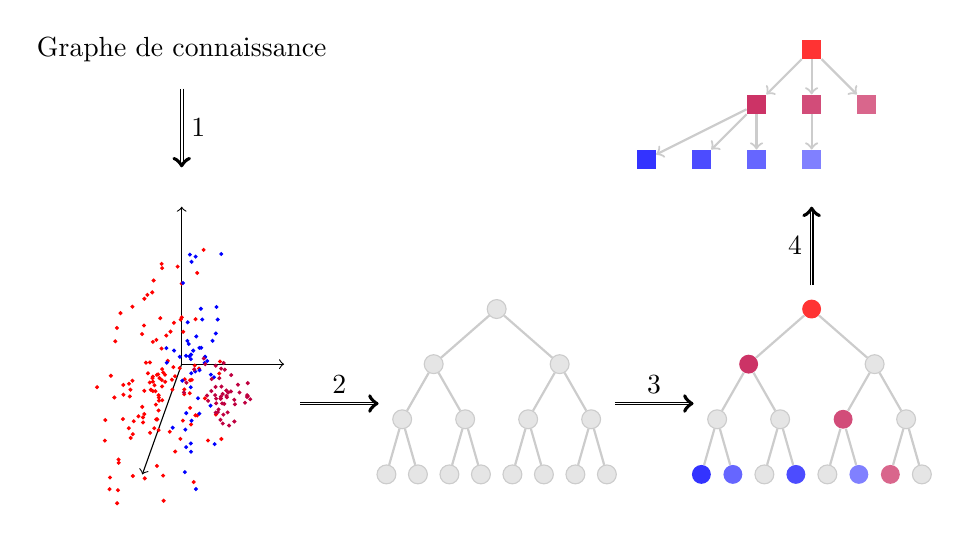
\begin{tikzpicture}
[   cnode/.style={draw=gray!40,fill=gray!20, minimum width=3mm, circle,inner sep=0.06, scale=0.8},
    colnode/.style={fill=#1,minimum width=3mm,circle,inner sep=0.06, scale=0.8},
    rnode/.style={draw=#1!40,fill=#1!20,minimum width=6mm, minimum height=6mm, rectangle},
    cline/.style={gray!40,thick},
    recnode/.style={fill=#1,minimum width=3mm, minimum height=3mm, rectangle, scale=0.8}
]

%
%\node at (0, 4.5) {Input Data};
\node at (0, 4) {Graphe de connaissance};
%\node at (0, 4) {$\{(e_i, t_i)\}$};

\draw [->] (0, 0) -- (0, 2);
\draw [->] (0, 0) -- (1.3, 0);
\draw [->] (0, 0) -- (-0.5, -1.4);

\draw [red] plot [only marks, draw=red, mark=*, mark size=0.5, domain=0:2, samples=120] ({2*(rnd-0.5)*rnd-0.3},{4*(rnd-0.5)*rnd-0.2});

\draw [blue] plot [only marks, draw=red, mark=*, mark size=0.5, domain=0:2, samples=50] ({(rnd-0.5)*rnd+0.1},{4*(rnd-0.5)*rnd+0.1});

\draw [purple] plot [only marks, draw=red, mark=*, mark size=0.5, domain=0:2, samples=50] ({1*(rnd-0.5)*rnd+0.5},{1*(rnd-0.5)*rnd-0.4});

%\node [red] at (-1.5, -1.5) {$t_1$};
%\node [blue] at (1.7, 1) {$t_2$};
%\node [purple] at (1.5, -1.5) {$t_3$};

    \draw[->, double] (0, 3.5) to[right] node {1} (0, 2.5);
    \draw[->, double] (1.5, -0.5) to[above] node {2} (2.5, -0.5);
    \draw[->, double] (5.5, -0.5) to[above] node {3} (6.5, -0.5);
    \draw[->, double] (8, 1) to[left] node {4} (8, 2); 

    % CLUSTERING %
    \def\offsetxa{4};
    \def\stepx{0.4};
    \def\stepy{0.7};
    
    \node[cnode] (000) at (-0.5*\stepx+\offsetxa,-2*\stepy) {};
    \node[cnode] (001) at (-1.5*\stepx+\offsetxa,-2*\stepy) {};
    \node[cnode] (010) at (-2.5*\stepx+\offsetxa,-2*\stepy) {};
    \node[cnode] (011) at (-3.5*\stepx+\offsetxa,-2*\stepy) {};
    \node[cnode] (100) at (0.5*\stepx+\offsetxa,-2*\stepy) {};
    \node[cnode] (101) at (1.5*\stepx+\offsetxa,-2*\stepy) {};
    \node[cnode] (110) at (2.5*\stepx+\offsetxa,-2*\stepy) {};
    \node[cnode] (111) at (3.5*\stepx+\offsetxa,-2*\stepy) {};
    
    \node[cnode] (00) at (-3*\stepx+\offsetxa,-\stepy) {};
    \node[cnode] (01) at (-1*\stepx+\offsetxa,-\stepy) {};
    \node[cnode] (10) at (1*\stepx+\offsetxa,-\stepy) {};
    \node[cnode] (11) at (3*\stepx+\offsetxa,-\stepy) {};
    
    \node[cnode] (0) at (-2*\stepx+\offsetxa,0*\stepy) {};
    \node[cnode] (1) at (2*\stepx+\offsetxa,0*\stepy) {};
    
    \node[cnode] (root) at (\offsetxa,\stepy) {};
    
    \draw[cline] (root) -- (0) {};
    \draw[cline] (root) -- (1) {};
    
    \draw[cline] (00) -- (0) {};
    \draw[cline] (10) -- (1) {};
    \draw[cline] (01) -- (0) {};
    \draw[cline] (11) -- (1) {};
    
    \draw[cline] (01) -- (000) {};
    \draw[cline] (01) -- (001) {};
    \draw[cline] (00) -- (010) {};
    \draw[cline] (00) -- (011) {};
    \draw[cline] (10) -- (100) {};
    \draw[cline] (10) -- (101) {};
    \draw[cline] (11) -- (110) {};
    \draw[cline] (11) -- (111) {};
    
    % CLUSTERING 2 %
    \def\offsetxc{\offsetxa+4};
    \def\stepx{0.4};
    \def\stepy{0.7};
    
    \node[colnode=blue!70] (000) at (-0.5*\stepx+\offsetxc,-2*\stepy) {};
    \node[cnode] (001) at (-1.5*\stepx+\offsetxc,-2*\stepy) {};
    \node[colnode=blue!60] (010) at (-2.5*\stepx+\offsetxc,-2*\stepy) {};
    \node[colnode=blue!80] (011) at (-3.5*\stepx+\offsetxc,-2*\stepy) {};
    \node[cnode] (100) at (0.5*\stepx+\offsetxc,-2*\stepy) {};
    \node[colnode=blue!50] (101) at (1.5*\stepx+\offsetxc,-2*\stepy) {};
    \node[colnode=purple!60] (110) at (2.5*\stepx+\offsetxc,-2*\stepy) {};
    \node[cnode] (111) at (3.5*\stepx+\offsetxc,-2*\stepy) {};
    
    \node[cnode] (00) at (-3*\stepx+\offsetxc,-\stepy) {};
    \node[cnode] (01) at (-1*\stepx+\offsetxc,-\stepy) {};
    \node[colnode=purple!70] (10) at (1*\stepx+\offsetxc,-\stepy) {};
    \node[cnode] (11) at (3*\stepx+\offsetxc,-\stepy) {};
    
    \node[colnode=purple!80] (0) at (-2*\stepx+\offsetxc,0*\stepy) {};
    \node[cnode] (1) at (2*\stepx+\offsetxc,0*\stepy) {};
    
    \node[colnode=red!80] (root) at (\offsetxc,\stepy) {};
    
    \draw[cline] (root) -- (0) {};
    \draw[cline] (root) -- (1) {};
    
    \draw[cline] (00) -- (0) {};
    \draw[cline] (10) -- (1) {};
    \draw[cline] (01) -- (0) {};
    \draw[cline] (11) -- (1) {};
    
    \draw[cline] (01) -- (000) {};
    \draw[cline] (01) -- (001) {};
    \draw[cline] (00) -- (010) {};
    \draw[cline] (00) -- (011) {};
    \draw[cline] (10) -- (100) {};
    \draw[cline] (10) -- (101) {};
    \draw[cline] (11) -- (110) {};
    \draw[cline] (11) -- (111) {};

%\node at (4, 0) {\Large $\Longrightarrow$};

% TAXONOMY
    \def\offsety{4};
    \def\offsetxtaxo{\offsetxc};

    \def\skipx{0.7};
    \def\skipy{0.7};
    
    \node[recnode=red!80] (l11) at (\offsetxtaxo, \offsety) {};
    
    \node[recnode=purple!80] (l21) at (-1*\skipx+\offsetxtaxo, \offsety-1*\skipy) {};
    \node[recnode=purple!70] (l22) at (\offsetxtaxo, \offsety-1*\skipy) {};
    \node[recnode=purple!60] (l23) at (1*\skipx+\offsetxtaxo, \offsety-1*\skipy) {};
    
    \node[recnode=blue!80] (l31) at (-3*\skipx+\offsetxtaxo, \offsety-2*\skipy) {};
    \node[recnode=blue!70] (l32) at (-2*\skipx+\offsetxtaxo, \offsety-2*\skipy) {};
    \node[recnode=blue!60] (l33) at (-1*\skipx+\offsetxtaxo, \offsety-2*\skipy) {};
    \node[recnode=blue!50] (l34) at (\offsetxtaxo, \offsety-2*\skipy) {};
    
    \draw[->, gray!40, thick] (l11) -- (l21) {};
    \draw[->, gray!40, thick] (l11) -- (l22) {};
    \draw[->, gray!40, thick] (l11) -- (l23) {};
    \draw[->, gray!40, thick] (l21) -- (l31) {};
    \draw[->, gray!40, thick] (l21) -- (l32) {};
    \draw[->, gray!40, thick] (l21) -- (l33) {};
    \draw[->, gray!40, thick] (l22) -- (l34) {};
\end{tikzpicture}